\section{Overview}

The high-level signal processing module (HLSPM) formats and displays
the digital EEG signal produced by the signal conversion module into a
human-viewable format. The HLSPM is implemented entirely in
software. Any available software visualization tool may be used to
inspect or display the data files created by the signal conversion
software of Chapter~\ref{chap:sc}. 

The ADC-42 system comes bundled with high-quality visualization
software which may be downloaded from the Pico
site\footnote{http://www.picotech.com}. EEG traces presented were
created with either the PicoScope 5.6.0 software
suite\footnote{http://www.picotech.com/downloads.html} using
Windows~98 or
Gnu-plot\footnote{http://www.cs.dartmouth.edu/gnuplot\_info.html} using
Red-hat~Linux~6.2.


\section{Signal display examples}

\begin{figure}[htbp]
	\psfrag{t}[][]{time [s]}
	\psfrag{0}[][]{0}
	\psfrag{+}[][]{+5~V}
	\psfrag{-}[][]{-5~V}
	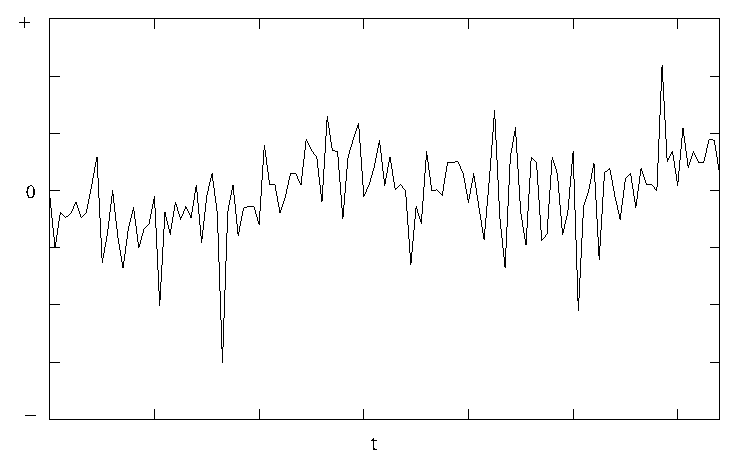
\includegraphics[width=\textwidth]{eeg-ex1.eps} 
	\caption{Raw EEG trace (1 second) }  
	\label{fig:eeg-ex2}
\end{figure}


Figure~\vref{fig:eeg-ex2} depicts a raw 1 second EEG trace. The
vertical amplitude scale represents a value between +5~V and -5~V
which is the full range of the signal conversion module output.  The
signal is marginally 'noisy' as judged by visual inspection of its
'spiky-ness'. Although a fairly vague description of signal
characteristics, qualitative descriptions of EEG traces seems to be
the norm in the literature. Where signals are averaged for several
iterations of the same stimuli more quantitative terms are used. The
graphic in Figure~\ref{fig:eeg-ex2} was generated using Gnu-plot.

\begin{figure}[htbp]
\begin{center}
	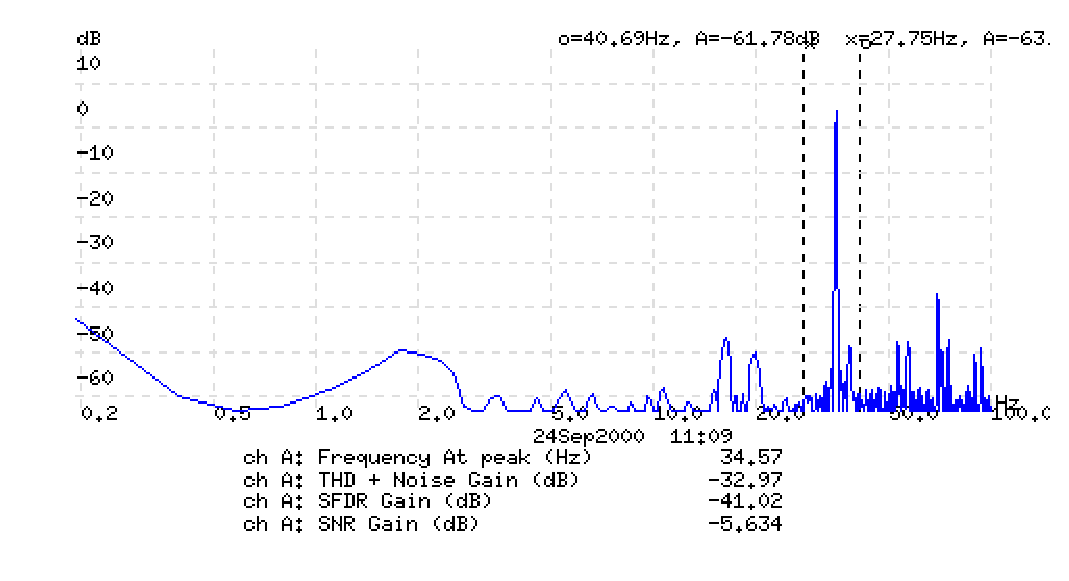
\includegraphics[width=\textwidth]{SME351.ps}
    \caption{SME 35~Hz ($\gamma$) source spectrum [dB/Hz]}
    \label{fig:sme35-1}
\end{center}
\end{figure}

Figure~\ref{fig:sme35-1} is another example of the output of the
high-level signal processing module. Here the FFT of a test signal
using the PicoScope software is calculated using the Hanning windowing
algorithm.
